% The discrete and integral terms disappear for different reasons.
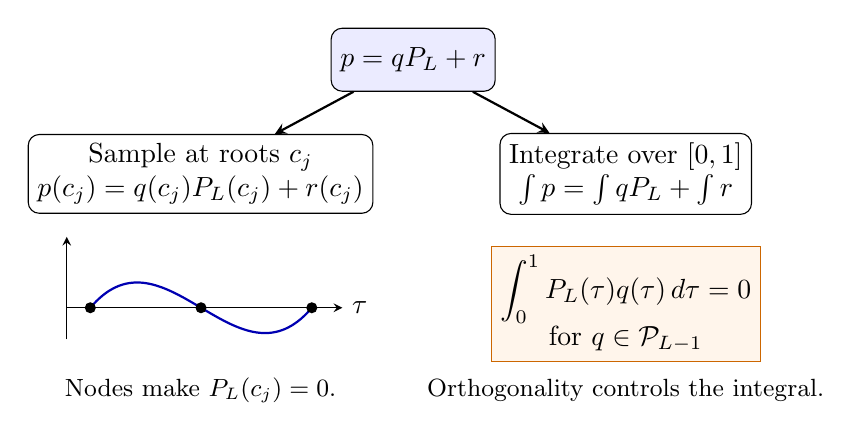
\begin{tikzpicture}[>=stealth,font=\normalsize,box/.style={draw,rounded corners,align=center,minimum height=.8cm}]
\node[box,fill=blue!8](p)at(0,1.9){$p=qP_L+r$};
\node[box](s)at(-2.7,.45){Sample at roots $c_j$\\$p(c_j)=q(c_j)P_L(c_j)+r(c_j)$};
\node[box](i)at(2.7,.45){Integrate over $[0,1]$\\$\int p=\int qP_L+\int r$};
\draw[->,thick](p)--(s);\draw[->,thick](p)--(i);
\draw[->](-4.4,-1.25)--(-.9,-1.25)node[right]{$\tau$};
\draw[->](-4.4,-1.65)--(-4.4,-.35);
\draw[blue!70!black,thick,domain=-4.1:-1.3,samples=70]plot(\x,{-1.25+.30*(\x+4.1)*(\x+2.694)*(\x+1.287)});
\foreach \x in {-4.1,-2.694,-1.287}{\fill(\x,-1.25)circle(2pt);}
\node[align=center,font=\small]at(-2.7,-2.3){Nodes make $P_L(c_j)=0$.};
\node[align=center,draw=orange!80!black,fill=orange!8]at(2.7,-1.2){$\displaystyle\int_0^1P_L(\tau)q(\tau)\,d\tau=0$\\for $q\in\mathcal P_{L-1}$};
\node[align=center,font=\small]at(2.7,-2.3){Orthogonality controls the integral.};
\end{tikzpicture}
